\documentclass{extarticle}
\sloppy

%%%%%%%%%%%%%%%%%%%%%%%%%%%%%%%%%%%%%%%%%%%%%%%%%%%%%%%%%%%%%%%%%%%%%%
% PACKAGES            																						  %
%%%%%%%%%%%%%%%%%%%%%%%%%%%%%%%%%%%%%%%%%%%%%%%%%%%%%%%%%%%%%%%%%%%%%
\usepackage[10pt]{extsizes}
\usepackage{amsfonts}
\usepackage{amsthm}
\usepackage{amssymb}
\usepackage{graphicx}
\usepackage[shortlabels]{enumitem}
\usepackage{microtype} 
\usepackage{amsmath}
\usepackage{mathtools}
\usepackage{commath}
\usepackage[margin=1in]{geometry}

%%%%%%%%%%%%%%%%%%%%%%%%%%%%%%%%%%%%%%%%%%%%%%%%%%%%%%%%%%%%%%%%%%%%%%
% PROBLEM ENVIRONMENT         																			           %
%%%%%%%%%%%%%%%%%%%%%%%%%%%%%%%%%%%%%%%%%%%%%%%%%%%%%%%%%%%%%%%%%%%%%
\usepackage{tcolorbox}
\tcbuselibrary{theorems, breakable, skins}
\newtcbtheorem{prob}% environment name
              {Problem}% Title text
  {enhanced, % tcolorbox styles
  attach boxed title to top left={xshift = 4mm, yshift=-2mm},
  colback=blue!5, colframe=black, colbacktitle=blue!3, coltitle=black,
  boxed title style={size=small,colframe=gray},
  fonttitle=\bfseries,
  separator sign none
  }%
  {} 
\newenvironment{problem}[1]{\begin{prob*}{#1}{}}{\end{prob*}}

%%%%%%%%%%%%%%%%%%%%%%%%%%%%%%%%%%%%%%%%%%%%%%%%%%%%%%%%%%%%%%%%%%%%%%
% THEOREMS/LEMMAS/ETC.         																			  %
%%%%%%%%%%%%%%%%%%%%%%%%%%%%%%%%%%%%%%%%%%%%%%%%%%%%%%%%%%%%%%%%%%%%%%
\newtheorem{thm}{Theorem}
\newtheorem*{thm-non}{Theorem}
\newtheorem{lemma}[thm]{Lemma}
\newtheorem{corollary}[thm]{Corollary}

%%%%%%%%%%%%%%%%%%%%%%%%%%%%%%%%%%%%%%%%%%%%%%%%%%%%%%%%%%%%%%%%%%%%%%
% MY COMMANDS   																						  %
%%%%%%%%%%%%%%%%%%%%%%%%%%%%%%%%%%%%%%%%%%%%%%%%%%%%%%%%%%%%%%%%%%%%%
\newcommand{\Z}{\mathbb{Z}}
\newcommand{\R}{\mathbb{R}}
\newcommand{\C}{\mathbb{C}}
\newcommand{\F}{\mathbb{F}}
\newcommand{\bigO}{\mathcal{O}}
\newcommand{\Real}{\mathcal{Re}}
\newcommand{\poly}{\mathcal{P}}
\newcommand{\mat}{\mathcal{M}}
\DeclareMathOperator{\Span}{span}
\newcommand{\Hom}{\mathcal{L}}
\DeclareMathOperator{\Null}{null}
\DeclareMathOperator{\Range}{range}
\newcommand{\defeq}{\vcentcolon=}
\newcommand{\restr}[1]{|_{#1}}


%%%%%%%%%%%%%%%%%%%%%%%%%%%%%%%%%%%%%%%%%%%%%%%%%%%%%%%%%%%%%%%%%%%%%%
% SECTION NUMBERING																				           %
%%%%%%%%%%%%%%%%%%%%%%%%%%%%%%%%%%%%%%%%%%%%%%%%%%%%%%%%%%%%%%%%%%%%%%
\renewcommand\thesection{\Alph{section}:}



%%%%%%%%%%%%%%%%%%%%%%%%%%%%%%%%%%%%%%%%%%%%%%%%%%%%%%%%%%%%%%%%%%%%%%
% DOCUMENT START              																			           %
%%%%%%%%%%%%%%%%%%%%%%%%%%%%%%%%%%%%%%%%%%%%%%%%%%%%%%%%%%%%%%%%%%%%%%
\title{\vspace{-2em}Chapter 4: Financial Markets}
\author{\emph{Summary}, by JF Viray}
\date{}

\begin{document}
\maketitle



%%%%%%%%%%%%%%%%%%%%%%%%%%%%%%%%%%%%%%%%%%%%%%%%%%%%%%%%%%%%%%%%%%%%%
% SECTION A            																			           
%%%%%%%%%%%%%%%%%%%%%%%%%%%%%%%%%%%%%%%%%%%%%%%%%%%%%%%%%%%%%%%%%%%%%
\section{Demand for Money ($M^d$)}
For the financial markets, you have the choice of either having money or bonds. For money, it is differentiated either through \textbf{currency} (coins and bills) and \textbf{checkable deposits} (bank deposits where you can use checks and credit cards). This distinction becomes important later on in Sections B and C where they prioritize currency and checkable deposits, respectively.

For bonds, you want them because they pay a positive interest rater $i$, but unlike money, you can't use them in transactions. Thus, you have a choice of how much money and bonds do you want to have, and this is dependent on the \textbf{level of transactions} and \textbf{interest rate on bonds}. We will focus on money market. Intuitively, if you transact more often, which we will represent through an increase in nominal income ($\$Y$), then you want more money. However, if the interest rates pay more on the bonds, then you would want less money. We would then model this demand for money ($M^d$) as:
$$M^d = \$Y \underset{(-)}{L(i)}$$
\section{Supply for Money ($M^S$) but Easy}
In any market, we need both demand and supply. Given we know demand for money, let's determine its supply. Suppose that all the money is just through the forms of currency, which only the central bank can print. Then, the supply of money ($M^S$) is determined by the central bank to be some amount $M$, and we thus have:
$$M^S = M$$
We can now have our equilibrium, and see that the interest rate is determined by the intersection between the demand and supply of the money market. 
\begin{figure}[h]
  \centering
  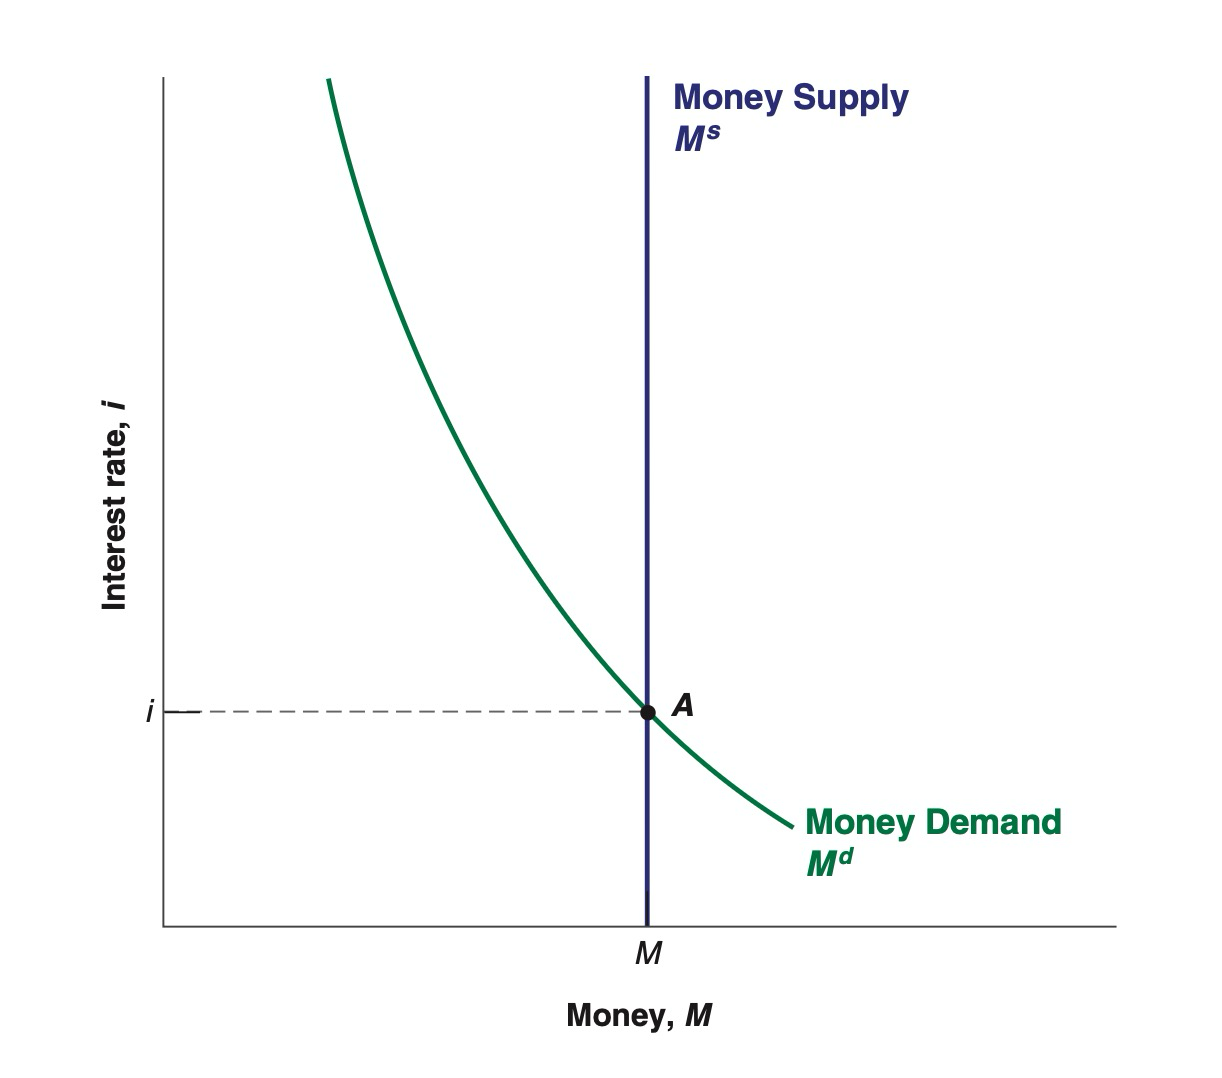
\includegraphics[width=0.5\linewidth]{money_market.png}
  \caption{Money Market}
  \label{fig:money}
\end{figure}

But, to actually change the money supply ($M^S$), the central bank goes to the bonds market and does its open market operations. If the central bank buys bonds, then it is called an expansionary open market operation because it expands the money supply. Conversely, if the central bank sells bonds, then it is called a contractionary open market operation because it contracts the money supply.

In the bonds market, what people actually use is the price of the bond ($P_B$), NOT the interest rate ($i$). However, if we suppose some promise of payment such as \$100, the interest rate ($i$) is a decreasing function of the bond price ($P_B$) by
$$i(\underset{(-)}{P_B}) = \frac{\$100 - \$P_B}{\$P_B}$$

As such, if the bond of the price goes up, then the interest rate ($i$) goes down. Let us now see what happens if the central bank buys bonds. Namely, two things happens in the money and bonds market; we show both implications.

$$\text{Buying Bonds} \implies \Delta M^{S^+}$$

$$\text{Buying Bonds} \implies \Delta \text{Demand for Bonds}^+ \implies \Delta P_B^+ \implies \Delta i^-$$

Thus, when the central bank buys bonds, it pays them with newly created money and thus have an increase in the money supply. 

\begin{figure}[h]
  \centering
  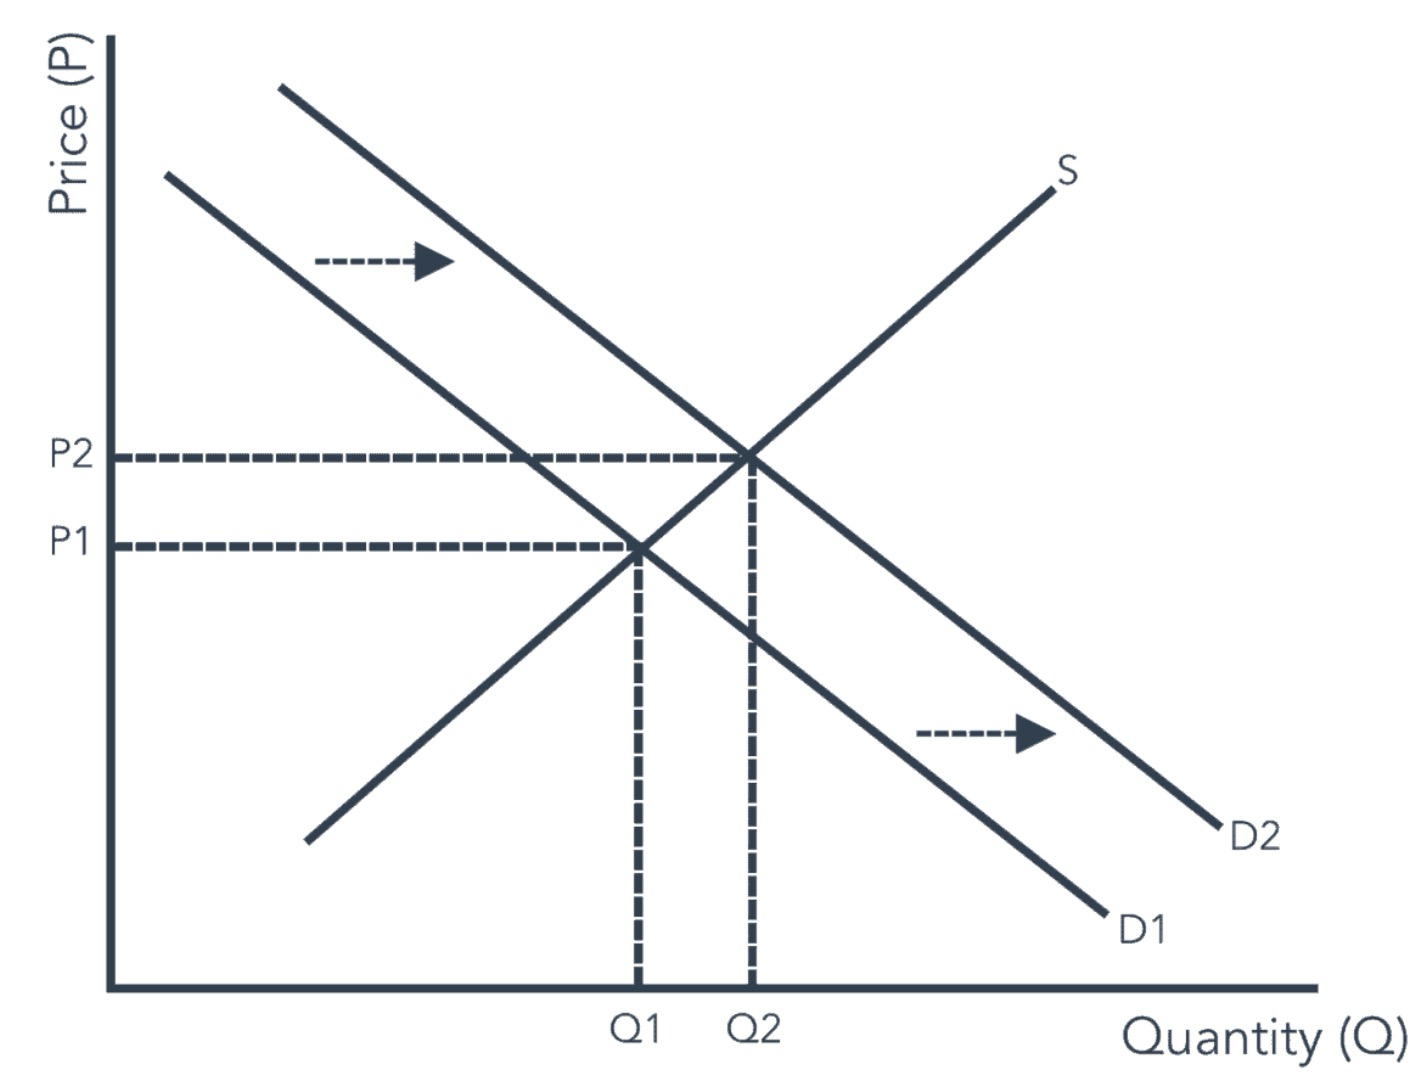
\includegraphics[width=0.5\linewidth]{bonds_market.png}
  \caption{An Increase in Demand in the Bonds Market}
  \label{fig:bonds}
\end{figure}

At the same time, the buying of bonds must mean the demand for bonds in the market increases. By our knowledge of microeconomics, an increase in demand implies an increase in price as per Figure 2. However, an increase in the price of bond means a decrease in the interest rate.

It is left as an exercise to the reader on how selling bonds by the central bank increases the interest rate and decreases the money supply.
\section{Supply for Money ($M^S$) but Hard}
Now, we let the banks enter into our model of the money market, so money is now in the form of either currency or checkable deposits. However, to make the algebra simpler, let's just assume all of the money is through the form of checkable deposits. We'll get the same general conclusion anyways~

Banks must keep reserves, both for precautionary reasons and due to legal requirements. Thus, the demand for central bank money has two parts: the demand for currency by people and the demand for reserves by banks. To simplify, we assume that people hold no currency, so the only demand for central bank money comes from banks. In this case, the demand for checkable deposits is the same as the demand for money:
$$M^d = \$YL(i)$$

Given this, the demand for reserves by banks is simply proportional to the demand
for checkable deposits. Let $\theta$ be the reserve ratio. Then:
$$H^d = \theta M^d = \theta \$Y L(i).$$

Finally, the central bank can choose the amount of money to supply, so we now have the equilibrium condition of
$$H = \theta \$Y L(i).$$
\begin{figure}[h]
  \centering
  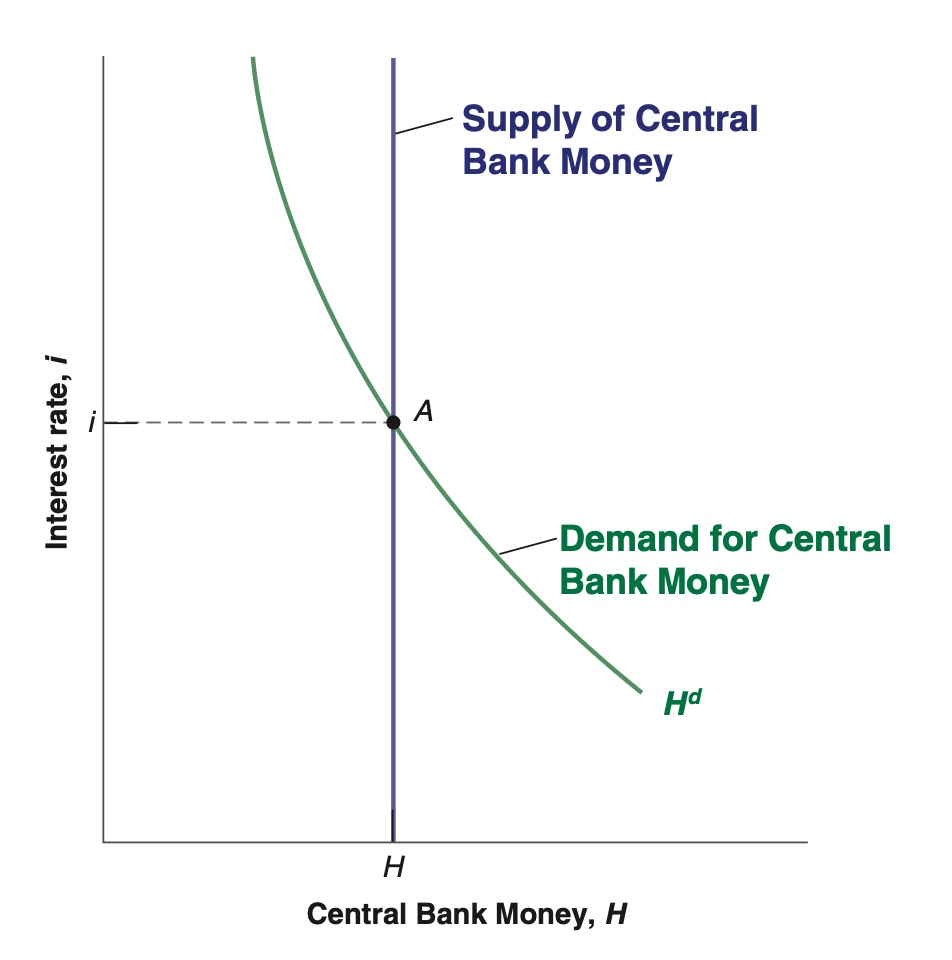
\includegraphics[width=0.3\linewidth]{central_bank.png}
  \caption{Market for Central Bank Money}
  \label{fig:central}
\end{figure}

\section{Liquidity Trap}
The interest rate cannot go below zero, a constraint known as the zero lower bound. When the interest rate is down to zero, monetary policy cannot decrease it further. Monetary policy no longer works, and the economy is said to be in a liquidity trap as shown in Figure 4.

\begin{figure}[h]
  \centering
  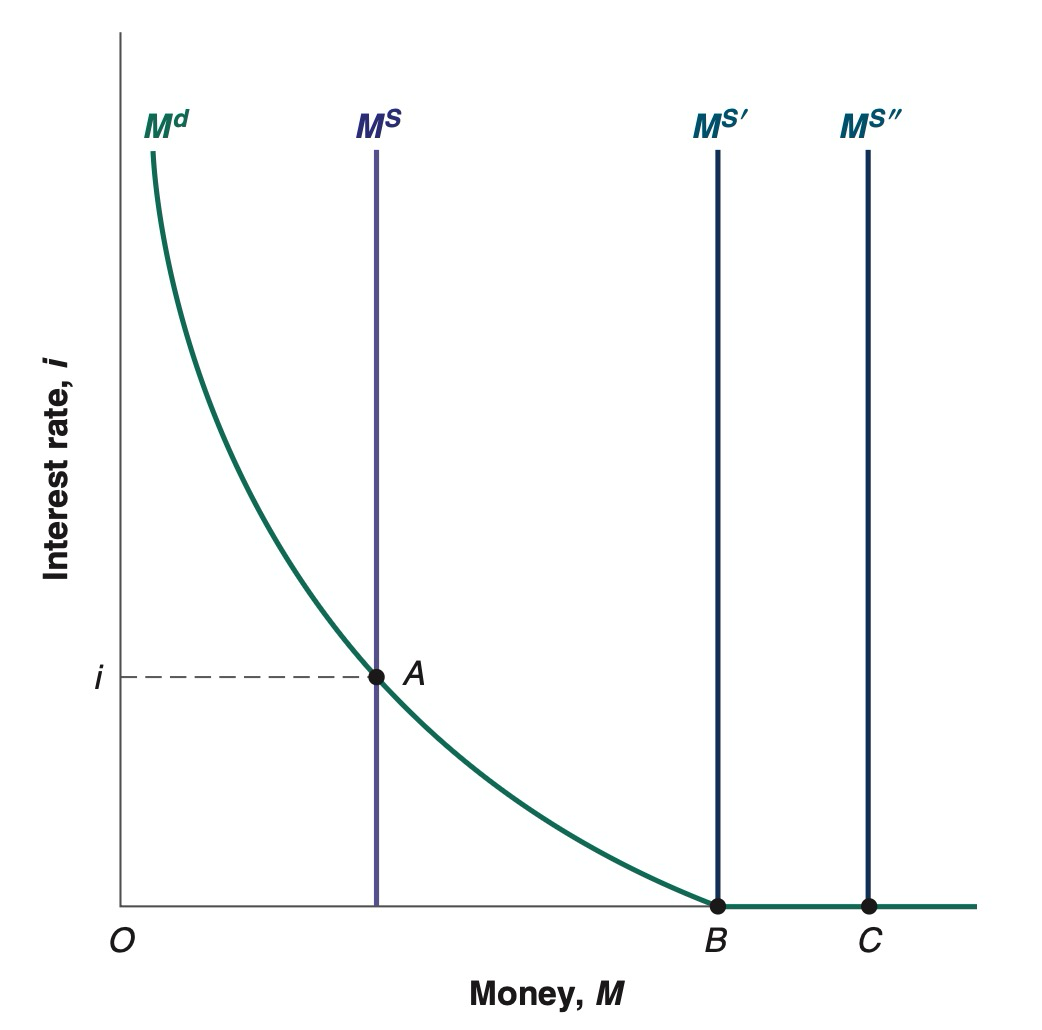
\includegraphics[width=0.3\linewidth]{liquidity_trap.png}
  \caption{Liquidity Trap}
  \label{fig:liquidity}
\end{figure}
\end{document}